
\subsection{Ecualizador de Fase}

En esta sección del informe se procederá a analizar un ecualizador de fase y control de tonos, cuyo circuito se presenta a continuación en la figura [\ref{circuito_ecualizador_de_fase}].


\begin{figure}[H]
	\centering
	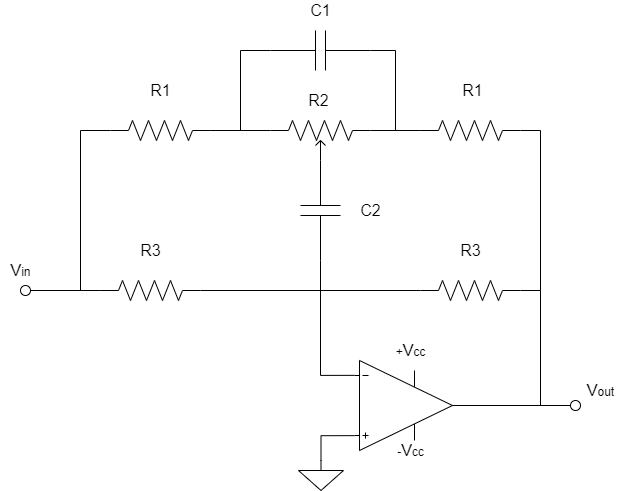
\includegraphics[width=0.45\textwidth]{../Ejercicio4-EcualizadorDeFase/Informe/Ecualizador_de_Fase.png}
	\caption{Circuito Ecualizador de Fase}
	\label{circuito_ecualizador_de_fase}
\end{figure}


\subsection{Análisis matemático}
A continuación, se presenta el desarrollo matemático pertinente para 
obtener la función transferencia del circuito planteado por la cátedra. \par 


Para analizar el circuito propuesto, se opto por reemplazar el potenciómetro $R_2$ 
por dos resistencias las cuales llamaremos 
$R_{21}$ y $R_{22}$, relacionadas por un coeficiente $L$. 
De esta forma será más fácil poder resolver el circuito propuesto, entonces definimos:

\vspace{1mm}
\begin{align}
		R_{21} &= R_2  L  \label{expresion_1} \\ 
		R_{22} &= R_2  (1 - L) \label{expresion_2}
\end{align}
\vspace{2mm}

Las relaciones entre ambas resistencias se plantean a continuación:

\vspace{2mm}
\begin{align}
	R_{21} + R_{22} &= R_2  L + R_2  (1 - L) = R_2 \label{suma_pote} \\ 	
	R_{21}  R_{22} &= R_2  L  R_2  (1 - L) = R_2^2(L-L^2)
	\label{multiplicacion_pote}
\end{align}
\vspace{2mm}

Usaremos las ecuaciones planteadas en [\ref{suma_pote}] y [\ref{multiplicacion_pote}] para 
simplificar las ecuaciones de la transferencia más adelante.


\begin{figure}[H]
	\centering
	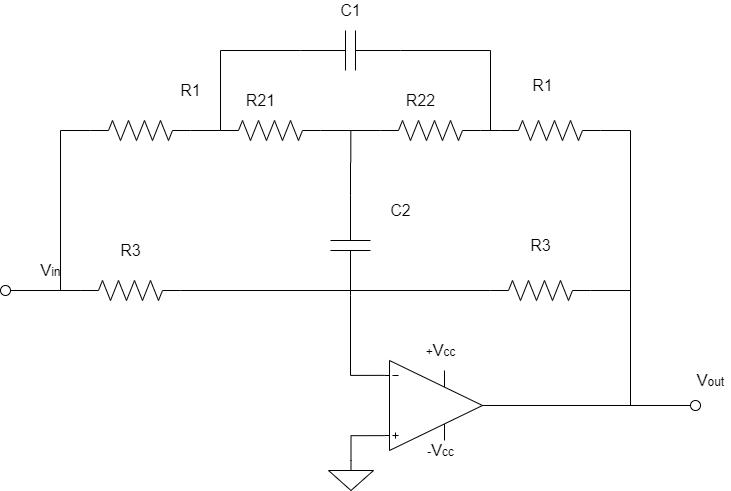
\includegraphics[width=0.45\textwidth]{../Ejercicio4-EcualizadorDeFase/Informe/EcSinPot.png}
	\caption{Modelo matemático}
\end{figure}
Para simplificar el circuito se procedió a aplicar las transformaciones 
de Kenelly en dos oportunidades. Primero, se procedió a una conversión 
triángulo-estrella para luego utilizar su contraparte estrella-triángulo. 
Este procedimiento  se muestra en las figuras [\ref{1reemplazo}]
  y [\ref{2reemplazo}]. \par 
Para el primer reemplazo se usaron las siguientes ecuaciones:

\begin{align*}
		Z_{AB} &= \frac{1}{sC_1} \\ 
		Z_{BC} &= R_{22} \\ 
		Z_{CA} &= R_{21}
\end{align*}
\vspace{2mm}

Considerando,

\begin{align*}
	Z_{eq} &= Z_{AB} + Z_{BC} + Z_{CA}
\end{align*}
\vspace{2mm}

Se procede a realizar la primera transformación de Kenelly.
 Obteniéndose: \par 

\begin{align}
	Z_{A} &= \frac{Z_{AB}+Z_{CA}}{Z_{eq}} \\
	Z_{B} &= \frac{Z_{AB}+Z_{BC}}{Z_{eq}}  \\
	Z_{C} &= \frac{Z_{BC}+Z_{CA}}{Z_{eq}} 
\end{align}
\vspace{2mm}

\begin{figure}[H]

	\centering
	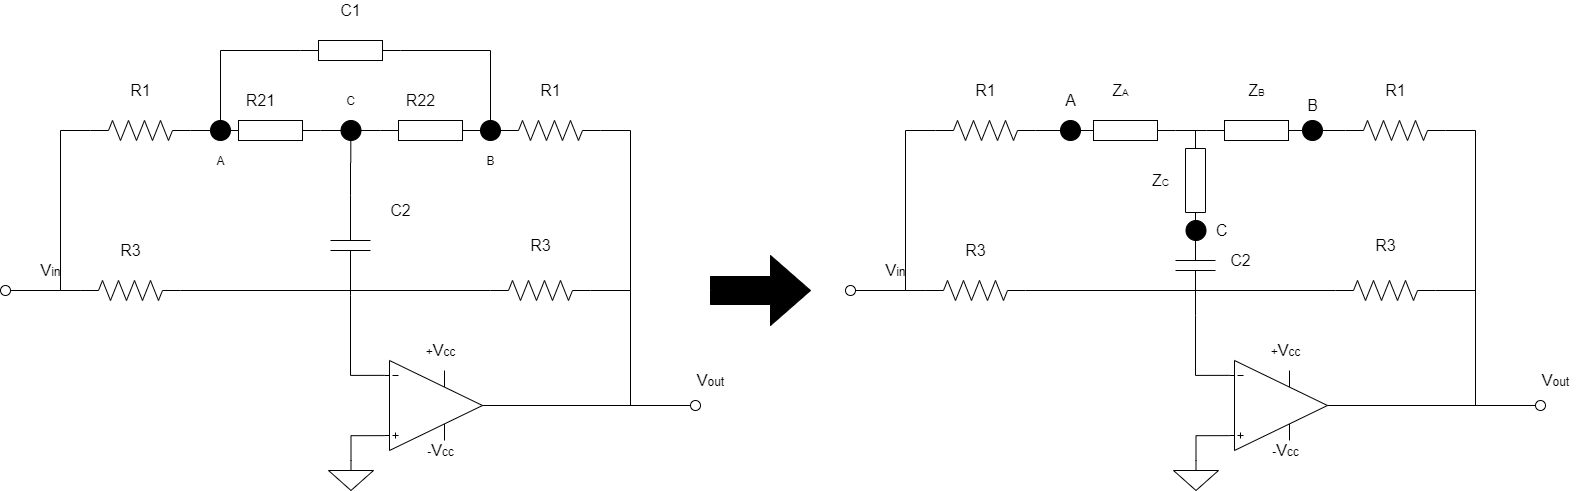
\includegraphics[width=0.9\textwidth]{../Ejercicio4-EcualizadorDeFase/Informe/1cambioEstrella.png}
	\caption{1° Reemplazo - Transformación estrella a triángulo}
	\label{1reemplazo} 
\end{figure}


Para el segundo reemplazo, se reagrupan las impedancias
 de la siguiente manera:
 \vspace{2mm}
\begin{align}
		Z_{A'} &= R_1 + Z_{A} \\
		Z_{B'} &= R_1 + Z_{B} \\
		Z_{C'} &= \frac{1}{sC_2} + Z_{C}
\end{align}
\vspace{2mm}
Se hacen las 
siguientes consideraciones:

\begin{align*}
	Z_{eq'} &= Z_{A'} + Z_{B'} + Z_{C'}
\end{align*}
\vspace{2mm}

Consecuentemente, se realiza la segunda transformación de Kenelly, pasando 
de un modelo estrella un triángulo. Obteniéndose las siguientes expresiones:

\begin{align}
	Z_{A'B'} &= \frac{Z_{eq'}}{Z_{C'}} \\
	Z_{B'C'} &= \frac{Z_{eq'}}{Z_{A'}}  \\
	Z_{C'A'} &= \frac{Z_{eq'}}{Z_{B'}} 
\end{align}
\vspace{2mm}


\begin{figure}[H]
	\centering
	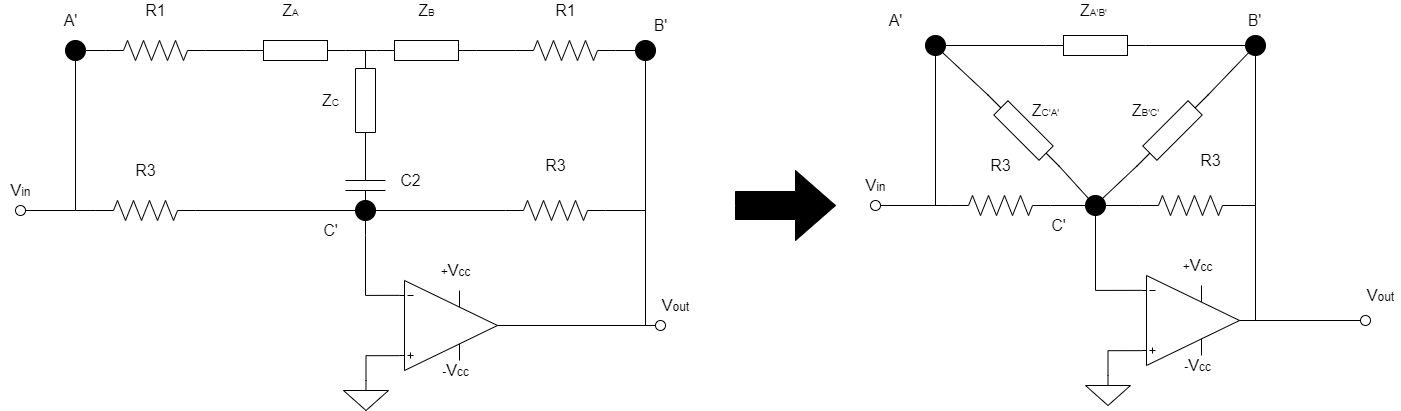
\includegraphics[width=0.9\textwidth]{../Ejercicio4-EcualizadorDeFase/Informe/2cambioTriangulo.png}
	\caption{2° Reemplazo - Transformación estrella a triángulo}
	\label{2reemplazo} 
\end{figure}

Por último, simplificamos las impedancias que estaban en paralelo obteniendo
 un circuito de 3 impedancias, representado por la figura
  [\ref{Cir_Final}], mucho más simple de resolver.

 \begin{align}
	Z_{1} & = Z_{C'A'}//R_3 \\
	Z_{2} & = Z_{B'C'}//R_3 \\ 
	Z_{3} & = Z_{A'B'}//R_3
\end{align} 
\vspace{2mm}

\begin{figure}[h]
	\centering
	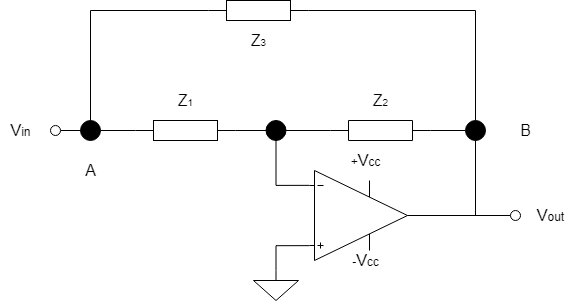
\includegraphics[width=0.45\textwidth]{../Ejercicio4-EcualizadorDeFase/Informe/EcFinal.png}
	\caption{Circuito simplificado}
	\label{Cir_Final}
\end{figure}

Debido al gran trabajo de cálculo requerido se decidió utilizar 
un programa matemático para asistirnos en el despeje de ecuaciones. 
El programa utilizado fue Matlab, del cual se desprenden las 
siguientes ecuaciones: \par 

\vspace{2mm}
\begin{align}
	Z_1 &= \frac{R_3(\alpha_1s^2+\alpha_2s+\alpha3)}{s^2(\alpha_1+C_1C_2R_1R_3R_{21}+C_1C_2R_1R_3R_{22})+s(\alpha_2+R_1R_3C_2+R_{22}R_3C_2)+\alpha_3} \label{z1} \\ 	
	Z_2 &= \frac{R_3(\alpha_1s^2+\alpha_2s+\alpha3)}{s^2(\alpha_1+C_1C_2R_1R_3R_{21}+C_1C_2R_1R_3R_{22})+s(\alpha_2+R_1R_3C_2+R_{21}R_3C_2)+\alpha_3} \label{z2} \\ 	
	Z_3 &= \frac{\alpha_1s^2+\alpha_2s+\alpha3}{s^2(C_1C_2R_{21}R_{22})+s(C_1R_{21}+C_1R_{22})+1} \label{z3}  	
\end{align}
\vspace{2mm}
Considerando las siguientes constantes:
\vspace{2mm}
\begin{align}
	\alpha_1 &= C_1C_2R_1^2R_{21}+C_1C_2R_1^2R_{22}+2C_1C_2R_1R_{21}R_{22}  \label{alpha1} \\ 	
	\alpha_2 &= 2C_1R_1R_{21}+2C_1R_1R_{22}+R_1^2C_2+R_1R_{21}C_2+R_1R_{22}C_2+R_{21}R_{22}C_2 \label{alpha2} \\ 	
	\alpha_3 &=  2R_1+R_{21}+R_{22}\label{alpha3}  	
\end{align}
\vspace{2mm}

Aplicando las expresiones obtenidas al principio de la seccción en 
[\ref{expresion_1}] y [\ref{expresion_2}], se pueden simplificar las ecuaciones 
[\ref{alpha1}],  [\ref{alpha2}] y [\ref{alpha3}] como:

\vspace{2mm}
\begin{align}
	\alpha_1 &= C_1C_2R_1^2R_2+2C_1C_2R_1R_2^2(L-L^2)  \label{alpha1_simplificado} \\ 	
	\alpha_2 &= 2C_1R_1R_2+R_1^2C_2+R_1R_2C_2+R_2^2(L-L^2)C_2 \label{alpha2_simplificado} \\ 	
	\alpha_3 &=  2R_1+R_2\label{alpha3_simplificado}  	
\end{align}
\vspace{2mm}

Por otro lado, utilizando las mismas expresiones se pueden simplificar las ecuaciones 
[\ref{z1}],  [\ref{z2}] y [\ref{z3}] como:

\vspace{2mm}
\begin{align}
	Z_1 &= \frac{R_3(\alpha_1s^2+\alpha_2s+\alpha3)}{s^2(\alpha_1+C_1C_2R_1R_3R_2)+s(\alpha_2+R_1R_3C_2+R_{22}R_3C_2)+\alpha_3} \label{z1_simplificado} \\ 	
	Z_2 &= \frac{R_3(\alpha_1s^2+\alpha_2s+\alpha3)}{s^2(\alpha_1+C_1C_2R_1R_3R_2)+s(\alpha_2+R_1R_3C_2+R_{21}R_3C_2)+\alpha_3} \label{z2_simplificado} \\ 	
	Z_3 &= \frac{\alpha_1s^2+\alpha_2s+\alpha3}{s^2(C_1C_2R_2^2(L-L^2))+s(C_1R_2)+1} \label{z3_simplificado}  	
\end{align}
\vspace{2mm}

A continuación, se realizarán dos análisis para obtener la función transferencia 
del circuito. La primera considerando un amplificador operacional ideal 
que implica las siguientes condiciones:

\begin{itemize}
	\item $A_{0}=\infty$
	\item $r_{in}=\infty$	
	\item $r_{o}=0$
\end{itemize}
De esta manera, se puede considerar una tierra virtual en la salida 
inversora del \textit{opamp}, obteniéndose la siguiente transferencia:

\begin{align}
	H_I(\$)=\frac{V_{out}}{V_{in}}=-\frac{Z_{2}}{Z_{1}}
	\label{trans_ideal}
\end{align}
 \vspace{2mm}

 Por otro lado, se analiza el caso de un \textit{opamp} no ideal, que 
 implica las siguientes condiciones:
 \begin{itemize}
	\item $A=\frac{A_{0}}{\left(1+\frac{s}{w_p}\right)}\neq\infty$
	\item $r_{in}\neq\infty$	
	\item $r_{o}\neq0$	
\end{itemize}
Este caso, al considerar menos aproximaciones, implica una mayor correlación 
con el funcionamiento empírico del circuito. Es necesario también 
utilizar las siguientes expresiones:

\begin{align}
	V_{out} & = A(V^+-V^-) \\
	V^+ & = 0 \\
	V^- & = V_{in} - I_1Z_1\\
	|I_1| & = \frac{V^-}{Z_{inp}} + \frac{V^--V_{out}}{Z_2}
\end{align} 
\vspace{2mm}

El circuito representado por dichas ecuaciones se puede apreciar 
en la figura [\ref{circuito_no_ideal}]. \par 
\begin{figure}[h]
	\centering
	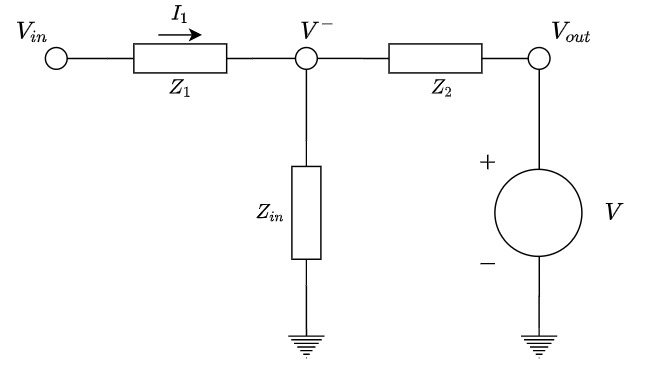
\includegraphics[width=0.45\textwidth]{../Ejercicio4-EcualizadorDeFase/Informe/circuito_no_ideal.png}
	\caption{Circuito resultante sin aproximaciones}
	\label{circuito_no_ideal}
\end{figure}


Finalmente, de las ecuaciones presentadas se puede despejar la transferencia 
no ideal del sistema como:

\begin{align}
	H_{NI}(\$)=\frac{V_{out}}{V_{in}}=\frac{A_0w}{Z_{1}Ys+w(Z_1Y-A_0\frac{Z_1}{Z_2})}
	\label{trans_no_ideal}
\end{align}
 \vspace{2mm}
Donde $Y$ está dado por:
\begin{align}
	Y=\frac{1}{Z_{in}}+\frac{1}{Z_1}+\frac{1}{Z_2}
	\label{Y}
\end{align}
 \vspace{2mm}

 A partir de [\ref{trans_no_ideal}] es posible llegar a [\ref{trans_ideal}] considerando:

 \begin{align}
	\lim_{A_0\to\infty} H_{NI}(\$) = H_{I}(\$)
	\label{Y}
\end{align}
 \vspace{2mm}

 Por ende, se considera la transferencia ideal para seguir despejando.

\begin{align}
	H_I(\$)=-\frac{Z_{2}}{Z_{1}}=-\frac{s^2(\alpha_1+C_1C_2R_1R_3R_2)+s(\alpha_2+R_1R_3C_2+R_{22}R_3C_2)+\alpha_3}{s^2(\alpha_1+C_1C_2R_1R_3R_2)+s(\alpha_2+R_1R_3C_2+R_{21}R_3C_2)+\alpha_3}
	\label{trans_ideal_aplicada}
\end{align}

 Por otro lado, con el fin de simplificar la transferencia obtenida
 se aplican las siguientes condiciones de diseño sobre la 
 ecuación [\ref{trans_ideal_aplicada}].

 \begin{equation}
	 R_3 \gg R_1 \hspace{4mm} \wedge \hspace{4mm} R_3=10R_2 \hspace{4mm} \wedge  \hspace{4mm} C_1=10C_2
 \end{equation}

 \vspace{2mm}

 Obteniéndose:
 \vspace{2mm}
 \begin{align}
	H(\$)=-\frac{\alpha_{1'}s^2+\alpha_{2'}s+\alpha_3}{\alpha_{1'}s^2+\alpha_{2''}s+\alpha_3}
	\label{trans_ideal_aplicada}
\end{align}
\vspace{2mm}
Donde las constantes están representadas por:

\vspace{2mm}
\begin{align}
	\alpha_{1'} &  \approx 20C_2^2R_1R_2^2(L-L^2) + 100C_2^2R_1R_2^2 \label{alpha1_prima} \\ 	
	\alpha_{2'} & \approx 31C_2R_1R_2+ C_2R_2^2(10-9L-L^2) \label{alpha2_prima} \\ 	
	\alpha_{2''} & \approx 31C_2R_1R_2+ C_2R_2^2(11L-L^2) \label{alpha2_primaprima}  	
\end{align}
\vspace{2mm}

Considerando la ecuación [\ref{trans_ideal_aplicada}], busco su variante normalizada 
para hallar la frecuencia de corte. 

\vspace{2mm}
\begin{align}
   H(\$)=-\frac{s^2\left(\frac{\alpha_{1'}}{\alpha_{3}}\right)+s\left(\frac{\alpha_{2'}}{\alpha_{3}}\right)+1}{s^2\left(\frac{\alpha_{1'}}{\alpha_{3}}\right)+s\left(\frac{\alpha_{2''}}{\alpha_{3}}\right)+1}
   \label{trans_ideal_aplicada_normalizada}
\end{align}
\vspace{2mm}

De [\ref{trans_ideal_aplicada_normalizada}] se puede despejar la frecuencia de corte del circuito
dada por:

\vspace{2mm}
\begin{align}
		\omega_0 &= \sqrt{\frac{\alpha_{3}}{\alpha_{1'}}} \\
		f_0 &= \frac{1}{2\pi} \sqrt{\frac{\alpha_{3}}{\alpha_{1'}}}    \label{w_0} 
\end{align}
\vspace{2mm}
Reemplazando [\ref{alpha1_prima}] y [\ref{alpha3_simplificado}] en [\ref{w_0}], se obtiene:

\vspace{2mm}
\begin{align}
		f_0 &= \frac{1}{2\pi} . \sqrt{ \frac{2R_1 + R_2 }{ 20 C_2^2 R_1 R_2^2 (L (1-L)) + 100R_1 R_2^2C_2^2 } }
\end{align}
\vspace{2mm}


\begin{equation}
	f_0 = \frac{1}{2\pi C_2 R_2} \sqrt{ \frac{2 + \frac{R_2}{R_1} }{ 20L(1-L) + 10 } }	
	\label{f0sinsimplificar}
\end{equation}
\vspace{3mm}

Considerando $10 \gg 20L(1-L)$, se obtiene la expresión propuesta por la cátedra.

\vspace{2mm}
\begin{equation}
		f_0 \approx \frac{ \sqrt{ 2 + \frac{R_2}{R_1} } }{ 20\pi C_2 R_2 }
		\label{f0final}
\end{equation}
\vspace{2mm}

Para finalizar el análisis se puede tomar la frecuencia de corte hallada 
y reemplazarla en el módulo de la función transferencia. De esta manera, 
tomando los valores extremos para $L$ se pueden obtener 
 las cotas para dicha función, 
dadas por la ecuación [\ref{A0cotas}].

\vspace{2mm}
\begin{equation}
		\frac{3R_1}{3R_1+R_2} \leq  A_0 \leq\frac{3R_1+R_2}{3R_1}
		\label{A0cotas}
\end{equation}
\vspace{2mm}


\subsection{Elección de componentes}
Para obtener una mejor simulación usamos 3 frecuencias debido a que el controlador de tonos debería usar frecuencias dentro del espectro audible para el oído humano, esto es en el rango de entre 20Hz y 20kHz, por lo que se debería predecir 3 valores de componentes para distintas frecuencias. Para frecuencias bajas donde están los sonido graves que están entre los 20Hz y 100Hz, para frecuencias medias donde se encuentran la una gran cantidad de sonidos musicales que están entre 400Hz y 900Hz, y para las frecuencias altas donde se encuentran los sonidos agudos suponemos un limite frecuencia ya que aunque el oído humano detecte hasta señales de 20kHz los sonidos que están por encima de los 5kHz ya no pertenecen a los generados por instrumentos musicales por lo que si suponemos un limite para nuestro circuito bien podría rondar entre los 5kHz y los 8kHz.
Para poder elegir los componentes y mantener la relaciones de simplificación ($C_1=10.C_2$ y $R_3=10.R_2$) tuvimos en cuanta que en el mercado solo hay valores nominales, por lo cual la elección se debía hacer en base a los componentes que se venden y no a lo que teóricamente queremos. El componente más determinante es el potenciómetro $R_2$ el cual tiene valores de venta mas restringidos, por ese mismo motivo utilizamos un potenciómetro de $10k\Omega$ y optamos por una relación de $R_2=10.R_2$ dándonos una resistencia de $R1=1k\Omega$. Luego buscamos mediante la ecuación \ref{f0final} valores de $C_2$ para frecuencias bajas, medias y altas ($50Hz$, $500Hz$ y $5kHz$ aproximadamente). Los valores de $C_2$ fueron los siguientes:

\begin{table}[h]
\centering
\begin{tabular}{|c|c|c|c|l}
\cline{1-4}
\textbf{Frecuencia deseada} & \textbf{$C_2$ deseado} & \textbf{$C_2$ comercial} & \textbf{Frecuencia obtenida} &  \\ \cline{1-4}
50Hz                        & 110nF                 & 100nF                   & 55Hz                         &  \\ \cline{1-4}
500Hz                       & 11nF                  & 10nF                    & 551Hz                        &  \\ \cline{1-4}
5kHz                        & 1.1nF                 & 1nF                     & 5.5kHz                       &  \\ \cline{1-4}
\end{tabular}
\end{table}

De los valores ya obtenidos a elección de $R_2$ y $C_2$ se calcularon las demás componentes con sus respectivas relaciones, siendo entonces la siguiente elección de componentes para las distintas frecuencias:

\begin{table}[htb]
\centering
\begin{tabular}{|c|c|c|c|c|c|}
\hline
\textbf{Frecuencia} & \textbf{$C_2$} & \textbf{$C_1$} & \textbf{$R_1$} & \textbf{$R_2$} & \textbf{$R_3$} \\ \hline
55Hz                & 100nF          & 1$\mu$F          & 1k$\Omega$     & 10k$\Omega$    & 100k$\Omega$   \\ \hline
551Hz               & 10nF           & 100nF           & 1k$\Omega$     & 10k$\Omega$    & 100k$\Omega$   \\ \hline
5.5kHz              & 1nF            & 10nF            & 1k$\Omega$     & 10k$\Omega$    & 100k$\Omega$   \\ \hline
\end{tabular}
\end{table}
\


\textbf{A TENER EN CUENTA}: Para tener mejores resultados en el circuito se debería usar tecnología SMD, que es tecnología de montaje superficial, ya que esta tecnología permite tener componentes resistivos con tolerancias de $1\%$ y capacitivos con $5\%$ logrando en la práctica mejores resultados. 


\subsection{Simulaciones}

Para las simulaciones se tuvo en cuenta que la posición del potenciómetro es lo que genera más variación sobre la transferencia en las distintas frecuencias, por lo que se mostrará las distintas simulaciones en posición de L=1 (donde $R_2$ es máximo), L=0.5 (donde $R_{21} = R_{22}$) y con L=0 (donde $R_2$ es mínimo) como casos extremos de cada frecuencia.

\subsubsection{Frecuencias bajas}
A continuación mostraremos las amplitudes en dB con los distintos valores de L simulados y teóricos. La frecuencia $f_0$ es de 55Hz.

\begin{figure}[H]
	\centering
	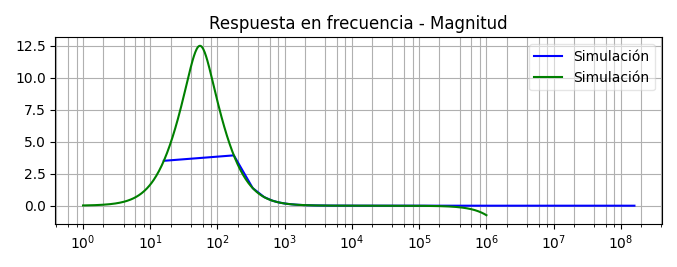
\includegraphics[width=0.6\textwidth]{../Ejercicio4-EcualizadorDeFase/Informe/lowFrecL000Mag.png} 
	\caption{Magnitud en dB con L=0}
	\label{lowMagL00}
\end{figure}
	
\begin{figure}[H]
	\centering
	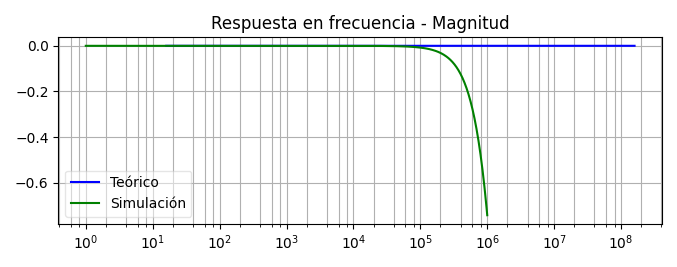
\includegraphics[width=0.6\textwidth]{../Ejercicio4-EcualizadorDeFase/Informe/lowFrecL050Mag.png} 
	\caption{Magnitud en dB con L=0.5}
	\label{lowMagL05}
\end{figure}

\begin{figure}[H]
	\centering
	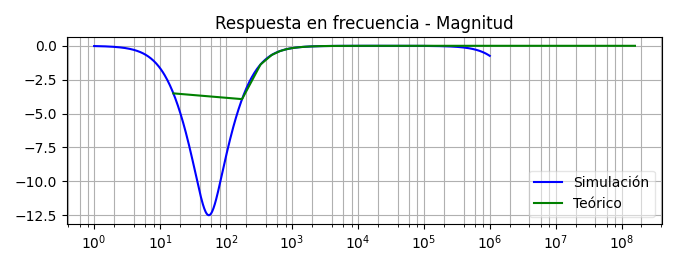
\includegraphics[width=0.6\textwidth]{../Ejercicio4-EcualizadorDeFase/Informe/lowFrecL100Mag.png} 
	\caption{Magnitud en dB con L=1}
	\label{lowMagL10}
\end{figure}


Ahora mostraremos las fases con los distintos valores de L simulados y teóricos.

\begin{figure}[H]
	\centering
	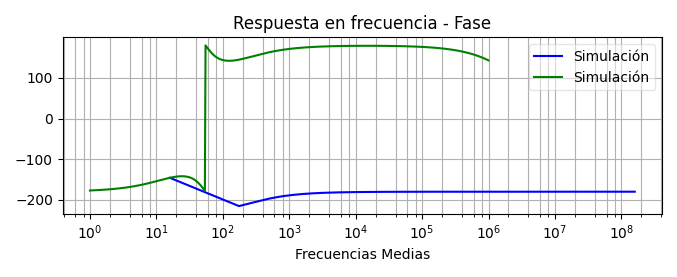
\includegraphics[width=0.6\textwidth]{../Ejercicio4-EcualizadorDeFase/Informe/lowFrecL000Fase.png} 
	\caption{Fase en grados con L=0}
	\label{lowFaseL00}
\end{figure}
	
\begin{figure}[H]
	\centering
	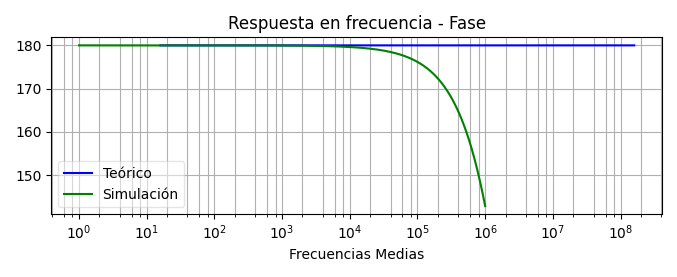
\includegraphics[width=0.6\textwidth]{../Ejercicio4-EcualizadorDeFase/Informe/lowFrecL050Fase.png} 
	\caption{Fase en grados con L=0.5}
	\label{lowFaseL05}
\end{figure}

\begin{figure}[H]
	\centering
	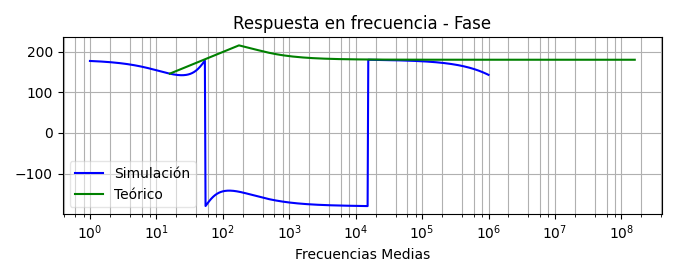
\includegraphics[width=0.6\textwidth]{../Ejercicio4-EcualizadorDeFase/Informe/lowFrecL100Fase.png} 
	\caption{Fase en grados con L=1}
	\label{lowFaseL10}
\end{figure}


\subsubsection{Frecuencias medias}
A continuación mostraremos las amplitudes en dB con los distintos valores de L simulados y teóricos. La frecuencia $f_0$ es de 551Hz.


\begin{figure}[H]
	\centering
	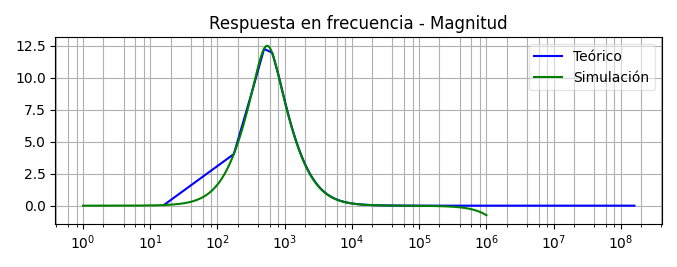
\includegraphics[width=0.6\textwidth]{../Ejercicio4-EcualizadorDeFase/Informe/medFrecL000Mag.png} 
	\caption{Magnitud en dB con L=0}
	\label{medMagL00}
\end{figure}
	
\begin{figure}[H]
	\centering
	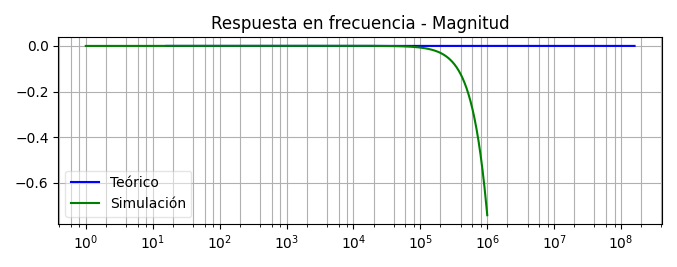
\includegraphics[width=0.6\textwidth]{../Ejercicio4-EcualizadorDeFase/Informe/medFrecL050Mag.png} 
	\caption{Magnitud en dB con L=0.5}
	\label{medMagL05}
\end{figure}

\begin{figure}[H]
	\centering
	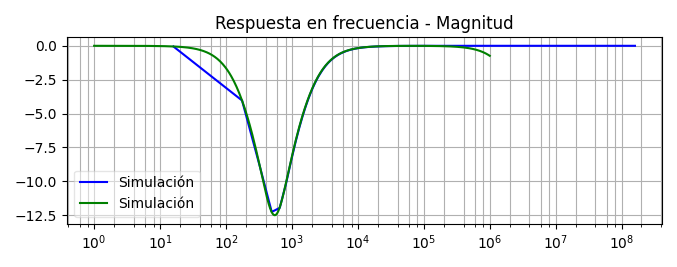
\includegraphics[width=0.6\textwidth]{../Ejercicio4-EcualizadorDeFase/Informe/medFrecL100Mag.png} 
	\caption{Magnitud en dB con L=1}
	\label{medMagL10}
\end{figure}


Ahora mostraremos las fases con los distintos valores de L simulados y teóricos.

\begin{figure}[H]
	\centering
	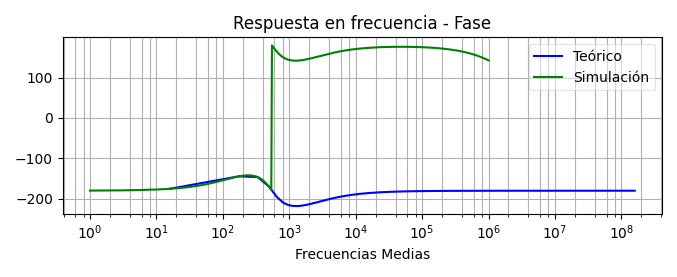
\includegraphics[width=0.6\textwidth]{../Ejercicio4-EcualizadorDeFase/Informe/medFrecL000Fase.png} 
	\caption{Fase en grados con L=0}
	\label{medFaseL00}
\end{figure}
	
\begin{figure}[H]
	\centering
	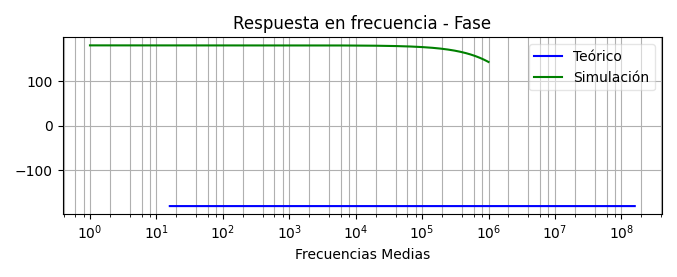
\includegraphics[width=0.6\textwidth]{../Ejercicio4-EcualizadorDeFase/Informe/medFrecL050Fase.png} 
	\caption{Fase en grados con L=0.5}
	\label{medFaseL05}
\end{figure}

\begin{figure}[H]
	\centering
	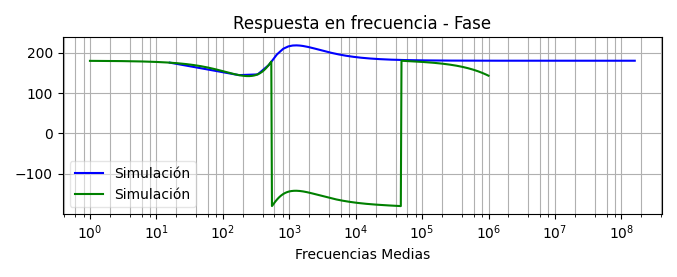
\includegraphics[width=0.6\textwidth]{../Ejercicio4-EcualizadorDeFase/Informe/medFrecL100Fase.png} 
	\caption{Fase en grados con L=1}
	\label{medFaseL10}
\end{figure}

\subsubsection{Frecuencias altas}
A continuación mostraremos las amplitudes en dB con los distintos valores de L simulados y teóricos. La frecuencia $f_0$ es de 5.5kHz.


\begin{figure}[H]
	\centering
	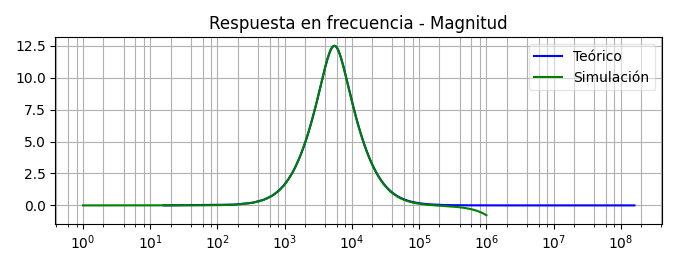
\includegraphics[width=0.6\textwidth]{../Ejercicio4-EcualizadorDeFase/Informe/highFrecL000Mag.png} 
	\caption{Magnitud en dB con L=0}
	\label{highMagL00}
\end{figure}
	
\begin{figure}[H]
	\centering
	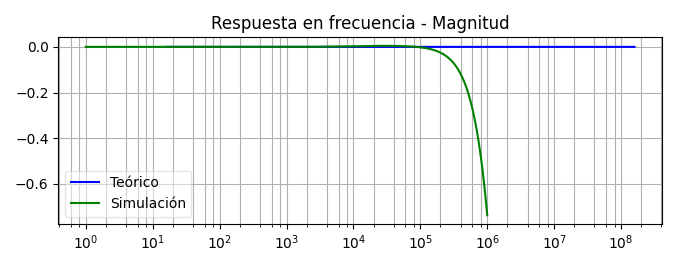
\includegraphics[width=0.6\textwidth]{../Ejercicio4-EcualizadorDeFase/Informe/highFrecL050Mag.png} 
	\caption{Magnitud en dB con L=0.5}
	\label{highMagL05}
\end{figure}

\begin{figure}[H]
	\centering
	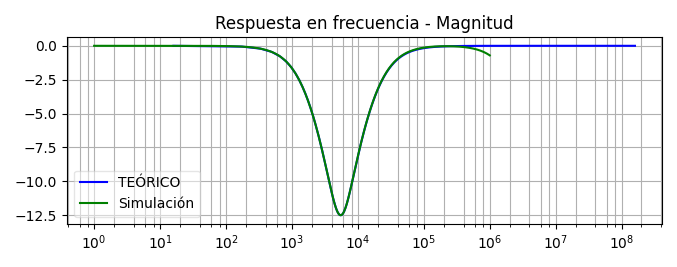
\includegraphics[width=0.6\textwidth]{../Ejercicio4-EcualizadorDeFase/Informe/highFrecL100Mag.png} 
	\caption{Magnitud en dB con L=1}
	\label{highMagL10}
\end{figure}


Ahora mostraremos las fases con los distintos valores de L simulados y teóricos.

\begin{figure}[H]
	\centering
	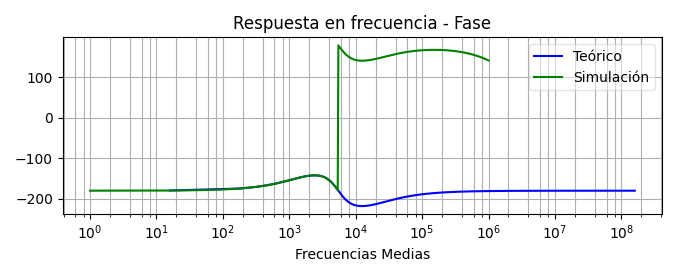
\includegraphics[width=0.6\textwidth]{../Ejercicio4-EcualizadorDeFase/Informe/highFrecL000Fase.png} 
	\caption{Fase en grados con L=0}
	\label{highFaseL00}
\end{figure}
	
\begin{figure}[H]
	\centering
	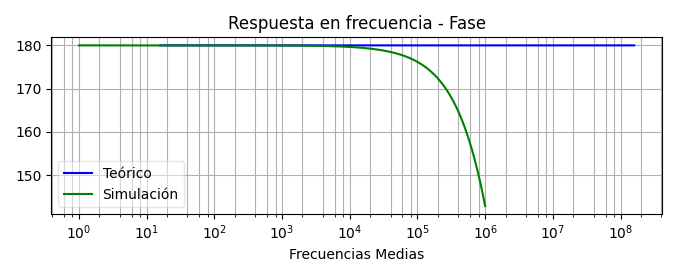
\includegraphics[width=0.6\textwidth]{../Ejercicio4-EcualizadorDeFase/Informe/highFrecL050Fase.png} 
	\caption{Fase en grados con L=0.5}
	\label{highFaseL05}
\end{figure}

\begin{figure}[H]
	\centering
	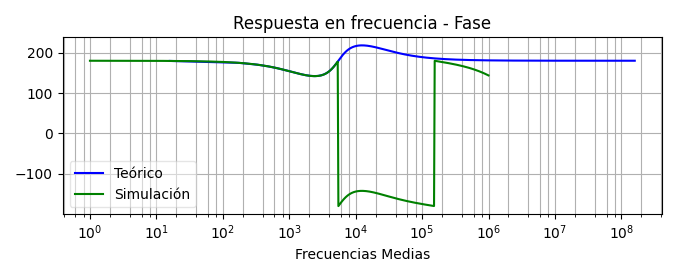
\includegraphics[width=0.6\textwidth]{../Ejercicio4-EcualizadorDeFase/Informe/highFrecL100Fase.png} 
	\caption{Fase en grados con L=1}
	\label{highFaseL10}
\end{figure}


De todas las simulaciones mostradas, tanto teóricas como por las del LTSpice, se puede notar como la posición del potenciómetro afecta a que las señales en $f_0$ se amplifiquen o se atenúen, esto es muy útil ya que la finalidad del controlador de tonos es poder elegir que tono quiero escuchar, si tuviera 3 bloques del mismo circuito (uno para cada frecuencia alta, media y baja) podría elegir a que frecuencia quiero escuchar o como balancear las 3 señales para generar la mejor armonía en mis sonidos de salida. 
También cabe destacar que las frecuencias mostradas fueron elegidas dentro 3 rangos amplios, podría hacerse varios circuitos para distintas frecuencias si lo que necesito son señales de determinadas frecuencias y no algo muy general, o contar con más de 3 bloques. Lo ideal sería conectar los bloques en cascada para que el ruido de un bloque no afecte a los demás.




